\subsection{État du jeu}
\begin{frame}{État du jeu}
	{\texttt{*} signifie constant} % Ça fait bizarre là où c'est mais ça gêne pas
	\begin{columns}
		\begin{column}{0.5\textwidth}
			\begin{typeag}{...}
				\variable{vies}{entier}\\
			\end{typeag}
			
		\end{column}
		\begin{column}{0.5\textwidth}
			\begin{typeag}{...}
				\variable{positionX}{entier ou réel}\\
				\variable{positionY}{entier ou réel}
			\end{typeag}
		\end{column}
	\end{columns}
\end{frame}

\subsection{Configuration initiale du jeu}
\begin{frame}{Configuration initiale du jeu}
	\begin{typeag}{...}
		\variablei{vies}{5}\\
	\end{typeag}
\end{frame}

\subsection{Évolution de l'état du jeu}
\begin{frame}[fragile]{Boucle principale}
	\begin{lstlisting}
		while ( vies > 0 ) {
			// Recuperation des entrees
			// Traitement
			// Affichage a l'ecran
		}
		afficher("Vous devez attendre 8 ans avant de pouvoir rejouer !");
	\end{lstlisting}
\end{frame}

\begin{frame}{Deplacement - vérification}
	\begin{columns}
		\begin{column}{0.49\textwidth}
			\begin{block}{Vérification}
				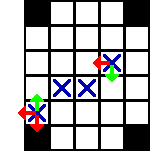
\includegraphics[width=\textwidth]{imgs/verifDepl}
			\end{block}
		\end{column}
		\begin{column}{0.49\textwidth}
			Vérifications :
			\begin{itemize}
				\item
					Déplacement dans la grille
				\item
					Déplacement sur case jouable
				\item
					Cases côtes à côtes
				\item
					Alignement de 3 ou plus
			\end{itemize}
		\end{column}
	\end{columns}
\end{frame}

\begin{frame}{Deplacement - détection et destruction}
	\begin{columns}
		\begin{column}{0.49\textwidth}
			\begin{block}{Détection}
				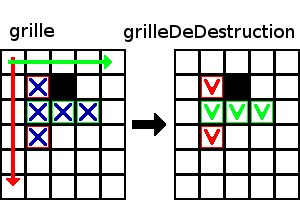
\includegraphics[width=\textwidth]{imgs/Detection}
			\end{block}
		\end{column}
		\begin{column}{0.49\textwidth}
			\begin{block}{Destruction}
				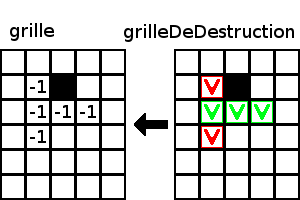
\includegraphics[width=\textwidth]{imgs/Destruction}
			\end{block}
		\end{column}
	\end{columns}
\end{frame}

\begin{frame}{Deplacement - remplacement}
	\begin{columns}
		\begin{column}{0.49\textwidth}
			\begin{block}{Tri des -1}
				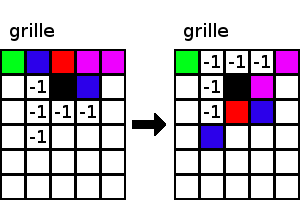
\includegraphics[width=\textwidth]{imgs/Remplacement1}
			\end{block}
		\end{column}
		\begin{column}{0.49\textwidth}
			\begin{block}{Tirage aléatoire des cases}
				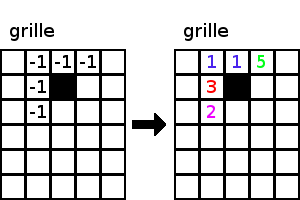
\includegraphics[width=\textwidth]{imgs/Remplacement2}
			\end{block}
		\end{column}
	\end{columns}
\end{frame}
